%
% Thesis - Main
% Lakshitha de Silva
% School of Computer Science
% University of St Andrews, Scotland, UK
% 2014
%

\documentclass{stacsthesis}

%
% Packages
%
\usepackage[english]{babel}
\usepackage{graphicx}
\usepackage{soul}
\usepackage{color}
\usepackage{tabulary}
\usepackage{booktabs}
\usepackage{listings}
\usepackage{enumitem}
\usepackage{pifont}
\usepackage[nointegrals]{wasysym}
\usepackage{syntax}
\usepackage{textcomp}
\usepackage[font=small,labelfont=bf,skip=16pt]{caption}
\usepackage{hyperref}
\usepackage[toc,acronym,nonumberlist,nomain]{glossaries}		% This has to load after hyperref package

%
% Compiler warnings
%
\hfuzz=10pt 
\vfuzz=10pt
\hbadness=10000
\vbadness=10000

%
% Configure code listings
%
\lstset {
	language=Java,
	basicstyle=\footnotesize\ttfamily\singlespacing,
	showstringspaces=false,
	keywordstyle=\color[RGB]{0, 0, 240},
	stringstyle=\color[RGB]{240, 0, 0},
	commentstyle=\color[RGB]{0, 144, 0},
	numberstyle=\tiny,
	basewidth=0.54em,
	tabsize=2,
	captionpos=b,
	frame=tb,
	framesep=10pt,
	aboveskip=8pt,
	belowskip=0pt,
	abovecaptionskip = 16pt,
	breakindent=24pt,
	breaklines=true,
	numberbychapter=true
}

%
% Console output
%
\lstdefinestyle{console} {
	language=bash,
	basicstyle=\footnotesize\ttfamily\singlespacing,
	backgroundcolor=\color[RGB]{248, 247, 242},
	upquote=true,
	frame=single,
	framerule=0pt,
	breakindent=0pt,
	breaklines=true,
	aboveskip=0pt,
	belowskip=4pt,
	xleftmargin=10pt,
	xrightmargin=10pt
}

%
% Inline coding listing commands
%
\def\javacode{\lstinline[basicstyle=\bfseries\ttfamily,basewidth=0.48em,language=Java]}

%
% Configure caption and sub-caption styles
%
\newsubfloat{figure}
\captionnamefont{\bfseries\small}
\captiontitlefont{\small}
\subcaptionlabelfont{\bfseries\footnotesize}
\subcaptionfont{\footnotesize}

%
% Customise titles names
%
\bibtitle{References}

%
% Customise toc
%
\maxtocdepth{subsection}

%
% Customise glossary
%
\renewcommand*{\glspostdescription}{}				% Remove dot at the end of glossary items
\makeglossaries								% Generate glossary

%
% Chapter and page style
%
\chapterstyle{stacs-chap}
\pagestyle{stacs-pg}

%
% Control word hyphenation
%
\hyphenpenalty=512
\tolerance=1024
\emergencystretch=4pt
\hyphenation{
	arti-ficial com-puter imple-ment imple-men-tation imple-men-ting frame-work
	Java
}

%
% Title page
%
\begin{document}
\hypersetup{pageanchor=false}
\title{Towards Controlling Software Architecture Erosion Through Runtime Conformance Monitoring}
\author{Lakshitha de Silva}
\school{School of Computer Science}
\degree{Doctor of Philosophy}
\submittextA{This thesis is submitted in partial fulfilment for the degree of}
\submittextB{at the University of St Andrews}
\submitdate{May 2014}
\maketitle

%
% Prologue
%
%
% Thesis - Abstract
% Lakshitha de Silva
% School of Computer Science
% University of St Andrews, Scotland, UK
% 2014
%


\begin{abstract}
Abstract goes here.
\end{abstract}

%
% Thesis - Acknowledgements
% Lakshitha de Silva
% School of Computer Science
% University of St Andrews, Scotland, UK
% 2014
%


\begin{acknowledgement}
Acknowledgements go here.
\end{acknowledgement}
%
% Thesis - Declarations
% Lakshitha de Silva
% School of Computer Science
% University of St Andrews, Scotland, UK
% 2014
%


\begin{declaration}
\subsection*{Candidate's Declarations}
I, \hl{<author>}, hereby certify that this thesis, which is approximately \hl{<word-count>} words in length, has been written by me, that it is the record of work carried out by me and that it has not been submitted in any previous application for a higher degree.

I was admitted as a research student and as a candidate for the degree of Doctor of Philosophy in \hl{September, 2009}; the higher study for which this is a record was carried out in the University of St Andrews between \hl{2009} and \hl{2013}.
\vspace{24pt}

Date:
\vspace{16pt}

Signature of candidate:
\vspace{48pt}


\subsection*{Supervisor's Declaration}
I hereby certify that the candidate has fulfilled the conditions of the Resolution and Regulations appropriate for the degree of Doctor of Philosophy in the University of St Andrews and that the candidate is qualified to submit this thesis in application for that degree.
\vspace{24pt}

Date:
\vspace{16pt}

Signature of supervisor:
\end{declaration}
%
% Thesis - Permission for electronic publication
% Lakshitha de Silva
% School of Computer Science
% University of St Andrews, Scotland, UK
% 2014
%


\begin{permission}
In submitting this thesis to the University of St Andrews I understand that I am giving permission for it to be made available for use in accordance with the regulations of the University Library for the time being in force, subject to any copyright vested in the work not being affected thereby. I also understand that the title and the abstract will be published, and that a copy of the work may be made and supplied to any bona fide library or research worker, that my thesis will be electronically accessible for personal or research use unless exempt by award of an embargo as requested below, and that the library has the right to migrate my thesis into new electronic forms as required to ensure continued access to the thesis. I have obtained any third-party copyright permissions that may be required in order to allow such access and migration, or have requested the appropriate embargo below.

The following is an agreed request by candidate and supervisor regarding the electronic publication of this thesis:

\begin{indentpara}
\emph{Access to printed copy and electronic publication of thesis through the University of St Andrews.}
\end{indentpara}

\vspace{24pt}

Date:
\vspace{16pt}

Signature of candidate:
\vspace{48pt}

Signature of supervisor:
\end{permission}
%
% Thesis - Dedication
% Lakshitha de Silva
% School of Computer Science
% University of St Andrews, Scotland, UK
% 2014
%


\begin{dedication}
Dedication goes here.
\end{dedication}
%
% Thesis - glossary and acronyms
% Lakshitha de Silva
% School of Computer Science
% University of St Andrews, Scotland, UK
% 2014
%


%
% Acronyms
%
\newacronym{vm}{VM}{virtual machine}
\newacronym{jvm}{JVM}{Java virtual machine}
\newacronym{jre}{JRE}{Java runtime environment}
\newacronym{cpu}{CPU}{central processing unit}
\newacronym{uml}{UML}{Unified Modelling Language}
\newacronym{ide}{IDE}{integrated development environment}
\newacronym{mvc}{MVC}{Model-View-Controller}



%
% Tables of contents/figures/tables and glossary
%
\cleardoublepage
\hypersetup{pageanchor=true}
\pagenumbering{roman}
\tableofcontents
\newpage\listoffigures
\newpage\listoftables
\newpage\lstlistoflistings
\printglossaries

%
% Mainmatter properties
%
\mainmatter
\onehalfspacing
\pagenumbering{arabic}
\setlength{\parskip}{3mm}
\setlength{\parindent}{0mm}
\setlist[enumerate]{leftmargin=*,labelsep=0.8em,topsep=0em,parsep=0.6em}
\setlist[itemize]{leftmargin=*,labelsep=1.0em,topsep=0em,parsep=0.6em,label=\normalsize\textbullet}
\newenvironment{itemize*}			% Itemising environment for single-lined items
	{\begin{itemize}					% Interline spacing has been adjusted in this case to
    		\setlength{\itemsep}{0.016em}}	% make the itemised text look more consistent with the rest
     	{\end{itemize}}

%
% Graphics directories
%
\graphicspath{
	{chap1/}
	{chap2/}
	{chap3/}
	{chap4/}
	{appA/}
	{appB/}
}

%
% Chapters
%
%
% Thesis - Chapter 1
% Lakshitha de Silva
% School of Computer Science
% University of St Andrews, Scotland, UK
% 2014
%


\chapter{Introduction}
<Chapter Abstract>

\section{Overview}


\section{Central claims}


\section{Motivation}


\section{Main contributions}


\section{Organisation of Dissertation}
A short description of each chapter in this thesis is given below.

\begin{description}
\item[Chapter 1] gives an introduction to this dissertation .. bla bla bla

\item[Chapter 2] presents the background survey .. bla bla bla
\end{description}


\section{Examples}

\subsection{Citing References}
References are used in the following paragraph.

Architecture erosion and its effects are widely discussed in literature. Perry and Wolf \cite{Perry1992} differentiate \emph{architecture erosion} from \emph{architecture drift} as follows: erosion results from violating architectural principles while drift is caused by insensitivity to the architecture. As the underlying causes for both are the same, we will not consider this difference for the purpose of our survey. Additionally, the notion of software architecture erosion is discussed using a number of different terms such as architectural degeneration \cite{Hoch2003}, software erosion \cite{Dalgar2009}, design erosion \cite{Gurp2002}, architectural decay \cite{Riaz2009}, design decay \cite{Izur2007}, code decay \cite{Eick2001,String2006} and software entropy \cite{Jacob1992}. 


\subsection{Tables}
Tables have been configured to use the \emph{booktabs} package which gives professionally typeset tables. Two examples are shown below.

\begin{table*}[h]\small
	\centering
	\begin{tabulary}{\textwidth}{lp{3pt}J}
		\toprule
		Strategy && Contribution towards controlling erosion \\
		\midrule
		Architecture Design Documentation & \RIGHTarrow & Records architecture design and rationale with the intent of disseminating architectural knowledge to a wider audience and provides a point of reference for developers throughout system evolution. \\ [7pt]
		Architecture Analysis & \RIGHTarrow & Uncovers weaknesses in the intended architecture, in particular, sensitive points which can be easily violated in the implementation.  \\ [7pt]
		Architecture Conformance Monitoring & \RIGHTarrow & Establishes the means to verify whether the implementation is faithful to the intended architecture during both the development and subsequent maintenance phases of a system. \\ [7pt]
		\bottomrule
	\end{tabulary}
	\caption{Controlling architecture erosion with process-oriented strategies}
	\label{tab:process-oriented}
\end{table*}

\begin{table}[h]
	\centering
	\begin{tabular}{llll} 
		\toprule
		Run 		& Framework unplugged ($\mu$s)	& Using probes	($\mu$s) & Using JDI ($\mu$s)	\\
		\midrule
		1		& 108,644			& 143,002				& 488,018		\\
		2		& 107,929			& 141,185				& 486,951		\\
		3		& 107,319			& 141,274				& 482,206		\\
		4		& 106,054			& 142,333				& 479,477		\\
		\midrule
		Average	& 107,487			& 141,949 (+30.9\%)		& 484,163 (+345.6\%)	\\
		\bottomrule
	\end{tabular}
	\caption{A comparison of performance impact between the use of JDI and instrumentation probes.}
	\label{tab:performance}
\end{table}


\newpage
\subsection{Lists}
An example of an itemised list.

\begin{itemize}
\item \textbf{Naming conventions from architectural to programming constructs.} For example, a component in the architecture is implemented by a class of the same name. Blah blah blah.

\item \textbf{Combining architecture and implementation in a single artefact.} Conformance checks are minimised or not required in such systems since architecture and implementation are combined in one specification.
\end{itemize}

An example of an enumerated list.

\begin{enumerate}
\item \textbf{Initialise the static analyser.} Provide the compiled Java code of the target application to Structure101 to begin its static analysis process.

\item \textbf{Analyse the Java bytecode.} Setup Structure101 to perform detailed analysis of the Java bytecode that also includes exploring method invocations among Java types.
\end{enumerate}


\subsection{Figures}
An example showing how to include figures. Figure \ref{fig:eventdriven} is taken from a pdf file which gives very good quality and therefore should be used for diagrams as much as possible.

\begin{figure}[h]
	\centering
	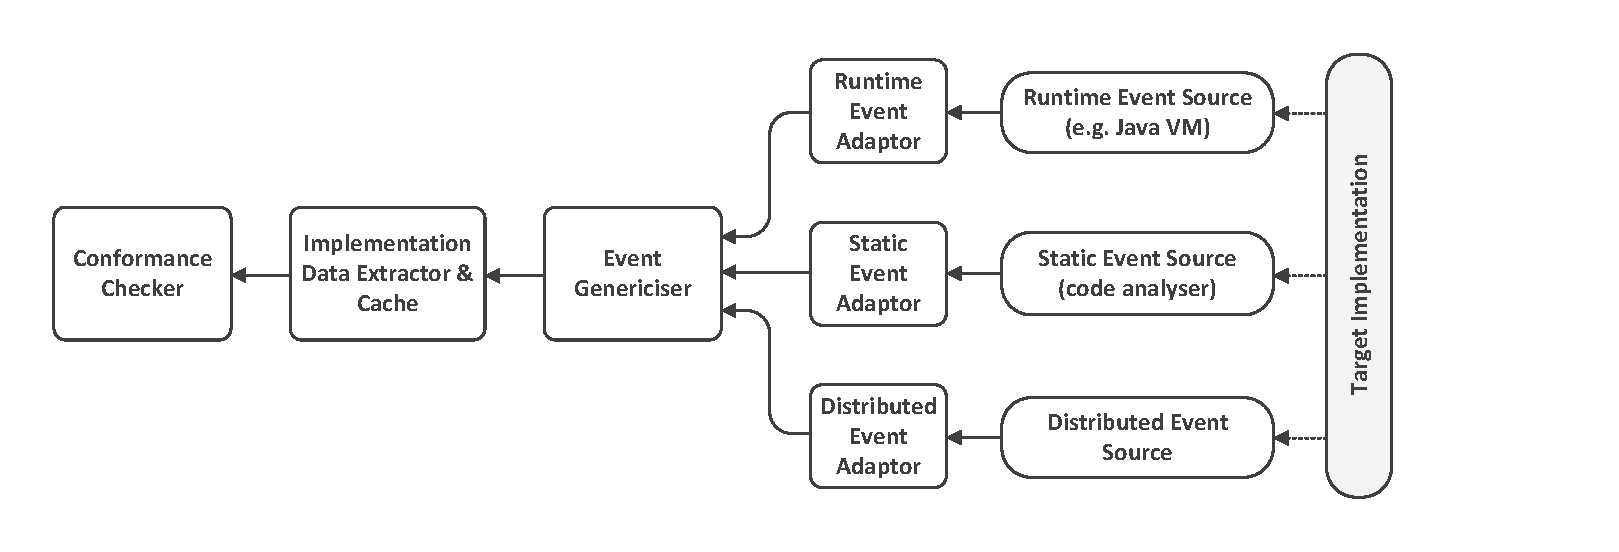
\includegraphics[width=\textwidth,trim=20 16 96 16]{fig-eventdriven.pdf}
	\caption{The event-driven process used for tapping implementation data}
	\label{fig:eventdriven}
\end{figure}


\newpage
\subsection{Code Listings}
An example of an inline code listing.
\begin{lstlisting}[caption={Hello World in Java},label=lst:javahello]
class HelloWorldApp {
	public static void main(String[] args) {
		System.out.println("Hello World!");		// Display messages
	}
}
\end{lstlisting}

Program code typeset from as an external file is shown in Listing \ref{lst:classtrans}. This also shows how to include line numbers.
\lstinputlisting[caption={Java class transformer},label=lst:classtrans,numbers=left]{
	chap1/src-example.java
}


\newpage
\subsection{Console Output}

\begin{lstlisting}[style=console]
John:/ $ ls -l
total 16437
drwxrwxr-x+ 52 root  admin     1768 10 Jan 13:21 Applications
drwxr-xr-x   3 root  wheel      102 27 Dec 18:01 Developer
drwxr-xr-x+ 66 root  wheel     2244  9 Jan 18:28 Library
drwxr-xr-x@  2 root  wheel       68 25 Aug 01:15 Network
drwxr-xr-x+  4 root  wheel      136 18 Dec 13:58 System
drwxr-xr-x   6 root  admin      204 18 Dec 14:16 Users
drwxrwxrwt@  4 root  admin      136 13 Jan 17:50 Volumes
drwxr-xr-x@ 39 root  wheel     1326 18 Dec 14:00 bin
drwxrwxr-t@  2 root  admin       68 25 Aug 01:15 cores
dr-xr-xr-x   3 root  wheel     4228 11 Jan 11:31 dev
lrwxr-xr-x@  1 root  wheel       11 18 Dec 13:46 etc -> private/etc
dr-xr-xr-x   2 root  wheel        1 13 Jan 16:10 home
-rwxr-xr-x@  1 root  wheel  8393256 20 Sep 06:22 mach_kernel
dr-xr-xr-x   2 root  wheel        1 13 Jan 16:10 net
drwxr-xr-x@  6 root  wheel      204 18 Dec 14:06 private
drwxr-xr-x@ 62 root  wheel     2108 18 Dec 14:02 sbin
lrwxr-xr-x@  1 root  wheel       11 18 Dec 13:47 tmp -> private/tmp
drwxr-xr-x@ 13 root  wheel      442 19 Dec 11:59 usr
lrwxr-xr-x@  1 root  wheel       11 18 Dec 13:47 var -> private/var
\end{lstlisting}


\subsection{Defining accronyms}
Blah blah blah \gls{vm} blah  blah blah blah and \gls{jvm}. However, blah blah blah, \gls{jvm} and also any other \gls{vm} blah blah blah. The \gls{jre} blah blah blah blah \gls{jvm} and blah blah blah blah \gls{cpu} blah blah blah blah blah. Typically, most blah blah blah \gls{ide} blah blah blah blah, however most \glspl{ide} blah blah blah blah blah blah blah.





%
% Thesis - Chapter 2
% Lakshitha de Silva
% School of Computer Science
% University of St Andrews, Scotland, UK
% 2014
%


\chapter{Context Survey}
\label{chap:background}
Numerous approaches have been proposed over the years either to prevent architecture erosion or to detect and restore eroded architectures. This chapter presents a survey of those approaches, which include techniques, tools and processes. They are classified primarily into three generic three categories that attempt to minimise, prevent and repair architecture erosion. Within these broad categories, each approach is further broken down  to reflect the high-level strategies adopted to tackle erosion. Some of these strategies in turn contain sub-categories under which survey results are presented. Merits and weaknesses of each strategy is discussed, with the argument that no single strategy can address the problem of erosion. The chapter concludes by presenting a case for further work in developing a holistic and practical approach for controlling architecture erosion.


\section{Introduction}
\subsection{Terminology}
\subsection{Other surveys}

\section{Classification}

\section{Discussion}

\section{Conclusions}

%
% Thesis - Chapter 3
% Lakshitha de Silva
% School of Computer Science
% University of St Andrews, Scotland, UK
% 2014
%



\chapter{Chapter 3 Title}
<Chapter Abstract>

\section{Overview}


\section{Section-2}


\section{Section-3}


\section{Conclusions}

%
% Thesis - Chapter 4
% Lakshitha de Silva
% School of Computer Science
% University of St Andrews, Scotland, UK
% 2014
%


\chapter{Chapter 4 Title}
<Chapter Abstract>

\section{Overview}


\section{Section-2}


\section{Section-3}


\section{Conclusions}


%
% Appendices
%
\appendix
%
% Thesis - Appendix A
% Lakshitha de Silva
% School of Computer Science
% University of St Andrews, Scotland, UK
% 2014
%



\chapter{Appendix-A Title}


%
% Thesis - Appendix B
% Lakshitha de Silva
% School of Computer Science
% University of St Andrews, Scotland, UK
%



\chapter{Appendix-B Title}


%
% Bibliography
%
\bibliographystyle{apalike}
\bibliography{thesis}

\end{document}
